\frame{
	\frametitle {Sigilo}
	\frametitle {Sigilo}
	\begin{figure}[ht]
	\begin{center}
	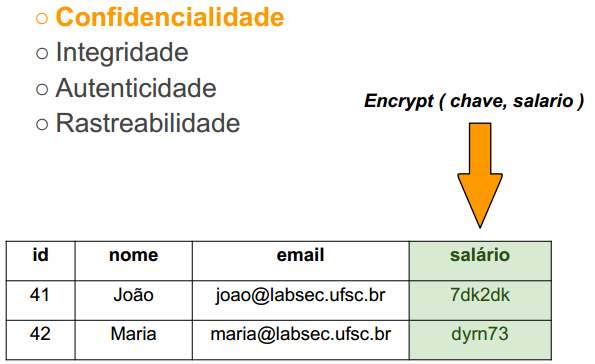
\includegraphics[width=\textwidth]{images/sigilo.png}
	\caption{Sigilo}
	\label{figura:sigilo}
	\end{center}
	\end{figure}
	
}

\frame{
	\frametitle {HMac}
	\begin{itemize}
	  \item Evitar a modificação não autorizada de registros contidos na base de dados.
	  \item Permite identificar as modificaçãos não autorizadas.
	\end{itemize}
		
}

\frame{
	\frametitle {HMac}
	
	\begin{figure}[ht]
	\begin{center}
	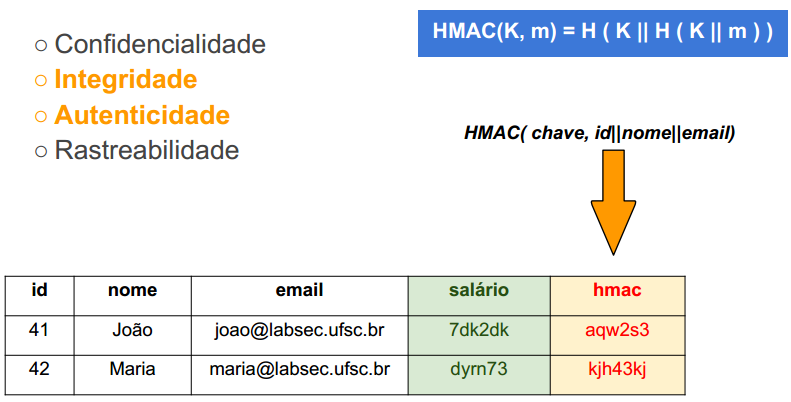
\includegraphics[width=\textwidth]{images/hmac.png}
	\caption{HMac}
	\label{figura:hmac}
	\end{center}
	\end{figure}
	
}

\frame{
	\frametitle {Histórico cifrado}
	\begin{itemize}
	  \item Com o HMac, não é possivel identificar remoções não autorizadas.
	  \item O Histórico Cifrado permite identificar as modificaçãos não autorizadas.
	  \item Permite relacionar dois ou mais registros de forma que possa se detectar a ausência de um deles.
	\end{itemize}

}

\frame{
	\frametitle {Histórico cifrado}
	\begin{itemize}
  	  \item Não permitir que uma terceira parte possa calcular o “histórico cifrado” sem conhecer as chaves de cifração.
  	  \item Utilização de operações de baixo custo computacional: criptografia simétrica e a operação lógica “ou exclusivo” (XOR);

	\end{itemize}

}

\frame{
	\frametitle {Histórico cifrado}
	
	\begin{figure}[ht]
	\begin{center}
	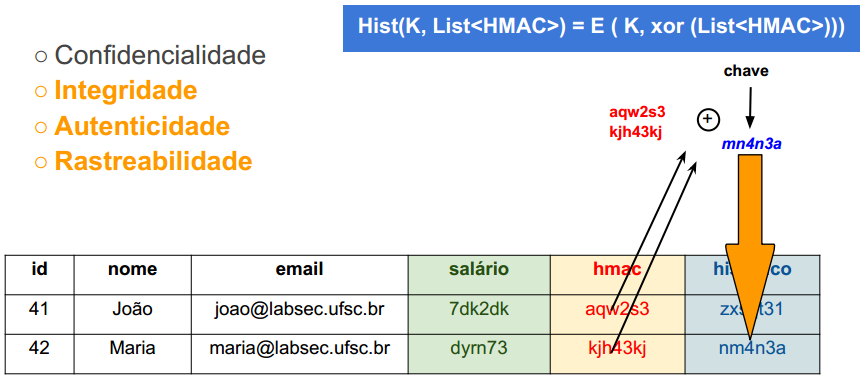
\includegraphics[width=\textwidth]{images/historico.png}
	\caption{Histórico Cifrado}
	\label{figura:historico}
	\end{center}
	\end{figure}

}
